\documentclass[a4paper,UKenglish]{lipics-v2018}
\usepackage{microtype}%if unwanted, comment out or use option "draft"
\bibliographystyle{plainurl}

\title{Formal Methods for Security - Final Report}

\author{Daniel Schaefer}{2549458}{}{}{}
\authorrunning{Daniel Schaefer}
\renewcommand{\copyrightline}{}

\begin{document}
\maketitle

\begin{abstract}
In this course we generally talked about various methods of model-checking security protocols. Later on here should be a text that summarizes the idea and findings of the seminar.\\
% TODO Extend

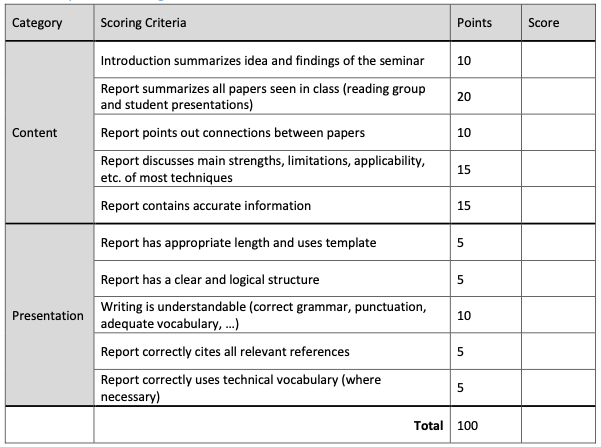
\includegraphics[scale = 0.72]{pictures/grading_scheme}\\
\end{abstract}


\newpage
\section{Model Checking Security Protocols}

This paper written by Basin et al. Outlines the difficulties of analyzing a security protocol in an automated fashion. The hardness of this particular problem specifically originates from the non-deterministic adversary, that is able to interact with arbitrary many protocol-executions that are being interleaved. Interaction with the executions in this case means, that the adversary is in control of the network that the protocol is executed on, which means that it can intercept, redirect and alter any data that is being sent.\cite{model_checking_security_protocols}

During et al. were able to proof that the secrecy problem is undecidable for such an attacker model if the number of protocol executions and random values (nonces) are unbounded.\cite{DLMS99} If one is able to keep the number of protocol executions bounded the secrecy problem was proven to be NP-complete by Rusinowitch and Turuani.\cite{RT01} This proof motivated development of model checkers in which the user explicitly specifies the number of protocol executions the model checker should search through which are in fact still useful in practice as most attacks on realistic protocols only require a few sessions.\cite{model_checking_security_protocols}

This attacker model is also called the Dolev-Yao attacker model. Many approaches of model checking cryptographic protocols adopted this attacker model and use it as part of an approach called 'Dolev-Yao symbolic model', which is explained in detail by Basin et al. in chapter 24.3 \cite{model_checking_security_protocols}.
% TODO: MAYBE: Pick important parts of definitions and list them here or a bit later maybe

In a symbolic model, messages are being represented by terms which formulate certain assumptions, essentially defining constraints on variables instead of arguing about concrete values. This measure is taken to counter the problem of state space explosion.\cite{model_checking_security_protocols}
% TODO: MAYBE: Define State space explosion?

% TODO: MAYBE: explain Notion of Secrecy and Weak Aliveness
% TODO: MAYBE: Forward vs Backwards Search?
% TODO: MAYBE: Link to computational soundness
% TODO: MAYBE: Non-Trace properties: e.g. non-interference, observational equivalence



\newpage
\section{Language Based Information Flow Security}

Sabelfeld at al. explain a promising new approach to guarantee that secret input data is not being 'leaked' to an attacker which observes the system output. This language-based technique, working on program semantics and analysis, relies on enforcing information-flow policies in source-code. Goal of these policies is to achieve properties like data confidentiality and noninterference.\cite{language_based_information_flow_security}

The approach, called "Information-flow control" is a mechanisms to enforce such policies. The analysis that is performed must then proof that no information flow exists, that would violate the previously specified policies.\cite{language_based_information_flow_security}

There are a significant number of channels one could leak information over, which are not directly transfering data. This is very obvious for the example of "termination channels" and "timing channels", which are related to an attackers ability to observe the behaviour of the program execution. This means that e.g. the duration of an computation or the non-termination of the program might leak information about secret values that were used as part of these computations.
The same applies to a number of additional channels, which are also not used to transfer data but still offer possible information leaks.\cite{language_based_information_flow_security} % TODO: List other Covert Channels

The focus in this paper is on a type checking approach to perform static information-flow analysis on compile time. Such a approach has already been implemented in the Jif compiler for Java.\cite{JFlow} The general idea is that a \textit{security type} is assigned to every program expression. This security type contains the ordinary type of the expression (such as int, float, string, etc.) and additionally a static label which describes how the resulting value can be used. This value is static and not determined on runtime, such that it can be used to verify the control flow on compile-time already.\cite{language_based_information_flow_security}
To be able to track implicit flows correctly, dependencies of the program-counter are additionally tracked.

The advantage of performing verification on compile time, compared to checking during runtime is that one is not limited to a single program execution, instead one can proof security of all possible program paths.\cite{language_based_information_flow_security}

% TODO: second half of this paper basically not contained in this summary
% TODO: Problems with this paper/approach



\newpage
\section{Secure Information flow by self-composition}
% TODO:



\newpage
\section{Automated Analysis of Cryptographic Protocols using Murphi}
% TODO:



\newpage
\section{SAT based model-checking for security protocol analysis}
% TODO:



\newpage
\section{Automatic Verification of Security Protocols in the Symbolic Model: the Verifier ProVerif}
Example citation \cite{ProVerif}
% TODO:



\bibliography{finalReport}


\end{document}
1